\chapter{صياغة الميكانيك الكمومي}\label{ch:b3:quantum-formalism}

خذ ثلاثة مرشّحات استقطاب. اثنان منها، متقاطعان عند $90^\circ$،
يحجبان الضوء حجبًا تامًّا؛ فأدخل الثالث بينهما عند $45^\circ$
يعبر الضوء \emph{من خلالها} --- فإضافة عائق تفتح الطريق.
ولا تصمد أمام هذه التجربة أيّ صورة للمرشّحات على أنها مناخل؛ والذي
يصمد هو الجبر الخطي: فاستقطاب الفوتون \emph{متجهة}،
وكل مرشّح يقيسه على محور ويسقطه،
والاحتمالات مربعات المركبات. ويرسي هذا الفصل
ذلك الجبر أساسًا فعليًا للميكانيك الكمومي. فالدوال
الموجية في الفصول السابقة لم تكن إلا ثوبًا ملموسًا واحدًا لجسد
أشدّ تجريدًا: فالحالات متجهات في \omterm{def:b3:quantum-formalism:state}{فضاء هيلبرت}،
والمرصودات مؤثرات هرميتية، والقيم المقيسة قيم ذاتية،
والاحتمالات مربعات جداءات سلّمية، والتطور مولَّد
\omterm{def:b3:hamiltonian-mechanics:hamiltonian}{بالهاميلتونية}. خمس مسلَّمات، كلها تعمل سلفًا في
كل ما حسبناه --- وهي، متى صيغت صياغة نظيفة، أقوى
من أن تعجز عن جمل لا تصفها موجة على مستقيم: استقطاب الفوتون،
وسبين الإلكترون، والنيوترينوات التي تتذبذب هويتها عبر الأرض.

\section{الحالات متجهات}

\begin{definition}[فضاء الحالات والكِتّات والأقواس]\label{def:b3:quantum-formalism:state}
\index{فضاء هيلبرت}\index{كِت}\index{برا}
تؤلف حالات جملة كمومية فضاءً متجهيًا عقديًا مزوَّدًا
بجداء داخلي --- أي \emph{فضاء هيلبرت} $\mathcal H$ (وتُطوَّر
رياضياته في كتاب رياضيات السنة الثالثة). والحالة
متجهة، تُكتب \emph{كِتًّا} $\ket\psi$، منظَّمة:
$\braket\psi\psi = 1$. والجداء الداخلي لحالتين هو العدد
العقدي $\braket\varphi\psi$، وهو خطي مرافق في الخانة الأولى،
مع $\braket\varphi\psi = \braket\psi\varphi^*$. وفي أساس
متعامد نظامي $\{\ket{e_i}\}$،
\[
\ket\psi = \sum_i c_i\ket{e_i} , \qquad
c_i = \braket{e_i}\psi , \qquad
\sum_i|c_i|^2 = 1 .
\]
والدالة الموجية في الفصول السابقة هي عائلة
مركبات $\ket\psi$ على المواضع: $\psi(x) =
\braket{x}{\psi}$؛ فلا يضيع شيء، وتصير الجمل ذات فضاءات
الحالات \emph{المنتهية} --- ولا يمكن حلمها أمواجًا --- قابلة للوصف.
\end{definition}

\begin{example}[استقطاب الفوتون: عالم ثنائي البعد]\label{ex:b3:quantum-formalism:polarization}
فوتون يمضي على المحور $z$ يحمل حالة استقطاب في \omterm{def:b3:quantum-formalism:state}{فضاء هيلبرت}
\emph{ثنائي} البعد، أساسه $\ket H$
(أفقي) و $\ket V$ (شاقولي). والضوء المستقطب بالزاوية
$\theta$ هو التراكب
\[
\ket\theta = \cos\theta\,\ket H + \sin\theta\,\ket V ,
\]
والاستقطاب الدائري هو التركيب العقدي $(\ket H \pm
\iu\ket V)/\sqrt2$: فكون المعاملات عقدية ليس زينة
بل فيزياء. وكل جملة كمومية ذات مستويين --- سبين أو جزيء
النشادر أو كيوبت فائق الناقلية --- هي هذا الفضاء المتجهي نفسه في
ثياب مختلفة.
\end{example}

\begin{omfigure}
\begin{tikzpicture}[font=\small, >=Stealth]
  \draw[->] (-0.3,0) -- (3.3,0) node[right] {$\ket H$};
  \draw[->] (0,-0.3) -- (0,3.3) node[above] {$\ket V$};
  \draw[->, omDef, very thick] (0,0) -- (35:2.9);
  \node[omDef, anchor=west] at (35:3.0) {$\ket\theta$};
  \draw[dashed, omThm] (35:2.9) -- ({2.9*cos(35)},0);
  \draw[dashed, omExo] (35:2.9) -- (0,{2.9*sin(35)});
  \node[omThm, anchor=north] at ({2.9*cos(35)},-0.08) {$\cos\theta$};
  \node[omExo, anchor=east] at (-0.08,{2.9*sin(35)}) {$\sin\theta$};
  \draw (1.0,0) arc (0:35:1.0);
  \node at (17:1.35) {$\theta$};
  \node[align=left, anchor=west] at (5.3,1.7)
    {الاحتمال على $\ket H$: $\cos^2\theta$\\[2pt]
     الاحتمال على $\ket V$: $\sin^2\theta$};
  \node[align=left, anchor=west, font=\footnotesize] at (5.3,0.45)
    {(قانون مالوس في كتاب السنة الأولى،\\مقروءًا من جديد قاعدةً لبورن)};
\end{tikzpicture}

{\small حالة استقطاب بوصفها متجهة: مربعات مركباتها على
أساس محلّل هي احتمالات النتائج --- أي هندسة صارت
احتمالًا.}
\end{omfigure}

\section{المرصودات مؤثرات}

\begin{definition}[المرصودات]\label{def:b3:quantum-formalism:observable}
\index{مرصودة}\index{مؤثر هرميتي}\index{قيمة ذاتية}
\emph{المرصودة} مؤثر خطي $\hat A$ على $\mathcal H$
يكون \emph{هرميتيًا}: أي $\braket{\varphi}{\hat A\psi} =
\braket{\hat A\varphi}{\psi}$ من أجل كل الحالات (وبلغة المصفوفات،
$A = A^{*\top}$). و\emph{متجهاته الذاتية} و\emph{قيمه الذاتية}،
$\hat A\ket{a} = a\ket{a}$، تحمل الفيزياء: فالقيم $a$ هي
القيم المقيسة الممكنة. ومن الحالات المألوفة: الموضع ($\hat x$:
الضرب في $x$)، وكمية الحركة ($\hat p = -\iu\hbar\,\dd/\dd x$)،
والطاقة ($\hat H = \hat p^2/2m + V(\hat x)$) --- وفي بُعدين،
أيّ مصفوفة هرميتية $2\times2$.
\end{definition}

\begin{theorem}[لماذا هرميتي]\label{thm:b3:quantum-formalism:hermitian}
\omterm{def:b3:quantum-formalism:observable}{للمؤثر الهرميتي} قيم ذاتية حقيقية، ومتجهاته الذاتية ذات
القيم الذاتية المتمايزة متعامدة؛ وعلى فضاءات هذا الكتاب تؤلف
متجهاته الذاتية أساسًا متعامدًا نظاميًا للفضاء $\mathcal H$ (وهي
\emph{المبرهنة الطيفية}، مبرهنةً في البعد المنتهي في كتاب رياضيات
السنة الثانية؛ أما من أجل المؤثرات غير المحدودة $\hat x$ و $\hat p$ و
$\hat H$ فالعبارة الكاملة تنتمي إلى النظرية الطيفية في السنة الثالثة وهي
مُسلَّم بها). فالقيم المقيسة يجب أن تكون حقيقية والنتائج المتمايزة
يجب أن تكون متعامدة: فالهرميتية هي بالضبط شرط أن يمثّل
مؤثرٌ قياسًا.
\end{theorem}

\begin{proof}[برهان جزئي]
$a\braket aa = \braket{a}{\hat Aa} = \braket{\hat Aa}{a} =
a^*\braket aa$: فالقيمة $a$ حقيقية. ومن أجل $\hat A\ket a = a\ket a$ و $\hat A\ket b
= b\ket b$: نجد $a\braket ba = \braket{b}{\hat Aa} = \braket{\hat
Ab}{a} = b\braket ba$، ومنه $(a - b)\braket ba = 0$.
\end{proof}

\begin{example}[مرصودة ذات مستويين]\label{ex:b3:quantum-formalism:twolevel}
على فضاء الاستقطاب، في الأساس $(\ket H, \ket V)$، لننظر في
\[
\hat A = \begin{pmatrix} 0 & 1\\ 1 & 0\end{pmatrix} :
\]
وهي هرميتية؛ وقيمها الذاتية $\pm1$؛ ومتجهاتها الذاتية $(\ket H \pm
\ket V)/\sqrt2$ --- أي الاستقطابان عند $\pm45^\circ$. وقياس
$\hat A$ \emph{يعني} السؤال ``قطري أم مضاد للقطري؟''، والأساس
الذاتي هو جوابا هذين السؤالين. وكل مستقطِب عند $45^\circ$
في التجربة الافتتاحية هو هذه المصفوفة في زجاج.
\end{example}

\section{المسلَّمات}

\begin{theorem}[قواعد الميكانيك الكمومي]\label{thm:b3:quantum-formalism:postulates}
\index{مسلَّمات الميكانيك الكمومي}\index{قاعدة بورن}\index{انهيار}
\emph{(م1)} حالة الجملة \omterm{def:b3:quantum-formalism:state}{كِت} منظَّم $\ket\psi$ في
\omterm{def:b3:quantum-formalism:state}{فضاء هيلبرت} الخاص بها.
\emph{(م2)} كل مقدار قابل للقياس \omterm{def:b3:quantum-formalism:observable}{مؤثر هرميتي}
$\hat A$.
\emph{(م3)} النتائج الممكنة الوحيدة لقياس $\hat A$ هي
قيمه الذاتية.
\emph{(م4)} على حالة $\ket\psi$، تقع النتيجة $a$ باحتمال
$\mathcal P(a) = |\braket a\psi|^2$ (وهي \omterm{thm:b3:quantum-formalism:postulates}{قاعدة بورن}؛ ومن أجل
\omterm{def:b3:quantum-formalism:observable}{قيمة ذاتية} منحلّة، تُجمع مربعات المركبات على
فضائها الذاتي). ومتوسط تجارب كثيرة هو $\langle\hat A\rangle =
\bra\psi\hat A\ket\psi$.
\emph{(م5)} بُعيد قياس أعطى $a$ مباشرةً، تكون الحالة
هي إسقاط $\ket\psi$ (منظَّمًا) على الفضاء الذاتي للقيمة $a$
--- وهو \emph{الانهيار}: فالقياس تفاعل يترك
الجملة في الحالة الموافقة لجوابه هو.
\emph{(م6)} بين قياسين تتطور الحالة تطورًا واحديًا وفق
معادلة شرودنغر
$\iu\hbar\,\dfrac{\dd}{\dd t}\ket{\psi(t)} = \hat H\ket{\psi(t)}$.
\end{theorem}
\admitted

\begin{example}[المستقطِبات الثلاثة، محسوبة]\label{ex:b3:quantum-formalism:threepolarizers}
ضوء شاقولي يلاقي محلّلًا متقاطعًا عند $90^\circ$: فيكون $|\braket
HV|^2 = 0$ --- أي انطفاء. فأدخل مستقطِبًا عند $45^\circ$: تعبره
الحالة $\ket V$ باحتمال $|\braket{45^\circ}{V}|^2 =
\tfrac12$ و\emph{تنهار} إلى $\ket{45^\circ}$ (بالمسلَّمة م5)؛ ثم تعبر تلك الحالة
المحلّلَ الأفقي باحتمال
$|\braket{H}{45^\circ}|^2 = \tfrac12$. فالنفوذ الصافي $\tfrac14$
بدل الصفر: فالمرشّح الأوسط لا ``يفتح ثقبًا'' --- بل
يؤدي قياسًا، ويعيد الانهيار تحضير الفوتون. ولا منخل
كلاسيكي يفعل هذا؛ والإسقاط لا يفعل غيره.
\end{example}

\begin{omfigure}
\begin{tikzpicture}[font=\small, >=Stealth]
  % light path
  \draw[->, omExo, very thick] (-0.9,0) -- (0.35,0);
  \draw[->, omExo, very thick] (0.65,0) -- (2.85,0);
  \draw[->, omExo, thick] (3.15,0) -- (5.35,0);
  \draw[->, omExo, thin] (5.65,0) -- (7.4,0);
  % polarizers
  \foreach \x/\ang/\lab in {0.5/90/{$V$}, 3.0/45/{$45^\circ$}, 5.5/0/{$H$}}
   {\draw[thick, fill=omDef!12] (\x,-1.05) ellipse (0.16 and 1.05);
    \draw[very thick, omDef] ($(\x,-1.05)+({\ang}:0.85)$) -- ($(\x,-1.05)-({\ang}:0.85)$);
    \node at (\x,-2.5) {\lab};}
  \node at (-0.9,0.45) {$I_0$};
  \node at (1.8,0.45) {$I_0$};
  \node at (4.3,0.45) {$I_0/2$};
  \node at (6.9,0.45) {$I_0/4$};
  \node[align=center, font=\footnotesize] at (3.0,1.5)
    {كل مرشّح يسقط الحالة على محوره:\\
     احذف الأوسط تصر الخرجة معدومة};
\end{tikzpicture}

{\small تجربة المستقطِبات الثلاثة بوصفها ثلاثة قياسات
متتالية: إسقاط ثم انهيار ثم إسقاط جديد. فمرشّح مضاف
\emph{يزيد} الضوء النافذ --- وهو مستحيل على المناخل،
تلقائي في الإسقاطات.}
\end{omfigure}

\begin{remark}[ما الذي لا يبيحه الانهيار]\label{rem:b3:quantum-formalism:nosignal}
الانهيار آنيّ في الصياغة، والارتباطات الكمومية
بين جسيمات متباعدة حقيقية ومقيسة --- لكن لا \emph{رسالة}
تركبها: فالنتائج عند كاشف واحد، مقروءةً وحدها، لا تُميَّز
من رمي قطعة نقد مهما فُعل بعيدًا. والعشوائية الكمومية غير
قابلة للردّ أيضًا: \omterm{thm:b3:quantum-formalism:postulates}{فقاعدة بورن} تعطي احتمالات حتى حين تكون الحالة
معلومة \emph{تمامًا} --- إذ لا شيء آخر يمكن معرفته. وكلتا العبارتين
مبرهنة من مبرهنات الصياغة، مختبَرة بدقة عالية؛ والانزعاج منهما
محترَم وقد قاد قرنًا من التجارب، ربح الميكانيكُ الكمومي كلَّ
واحدة منها.
\end{remark}

\section{المبدّلات والارتياب}

\begin{definition}[المبدّلة؛ المرصودات المتوافقة]\label{def:b3:quantum-formalism:commutator}
\index{مبدّلة}\index{مرصودات متوافقة}
\emph{مبدّلة} مؤثرين هي $[\hat A, \hat B] = \hat
A\hat B - \hat B\hat A$. والمثال المؤسِّس، انطلاقًا من $\hat p =
-\iu\hbar\,\dd/\dd x$:
\[
[\hat x, \hat p] = \iu\hbar .
\]
وتكون مرصودتان \emph{متوافقتين} حين $[\hat A, \hat B] = 0$:
فتقبلان عندئذٍ أساسًا ذاتيًا مشتركًا ويمكن معرفتهما معًا؛
وقياس إحداهما لا يزعج حالة حادّة في الأخرى. ومجموعة
مرصودات متبادلة يكون أساسها الذاتي المشترك وحيدًا (أي
\emph{CSCO}) هي ما يعنيه ``وسم حالة وسمًا تامًّا'' --- والوسوم
$(n_1, n_2, n_3)$ في العلبة كانت هذا بالضبط.
\end{definition}

\begin{theorem}[علاقة الارتياب في العموم]\label{thm:b3:quantum-formalism:uncertainty}
\index{علاقة الارتياب}
في أيّ حالة، يحقق الانحرافان المعياريان لمرصودتين
\[
\Delta A\;\Delta B \ \ge\ \tfrac12\,\big|\langle[\hat A, \hat
B]\rangle\big| .
\]
ومن أجل $\hat x$ و $\hat p$: $\Delta x\,\Delta p \ge \hbar/2$ ---
أي علاقة هايزنبرغ، وقد صارت الآن مبرهنة من الجبر الخطي لا
قاعدة تخمينية. فاللاتوافق كمّي: إذ يحدّد حجم \omterm{def:b3:quantum-formalism:commutator}{المبدّلة}
أرضية الحدّة المشتركة.
\end{theorem}

\begin{proof}[برهان جزئي]
ليكن $\hat\alpha = \hat A - \langle A\rangle$ و $\hat\beta = \hat B -
\langle B\rangle$. تعطي متراجحة كوشي--شوارتز في كتاب رياضيات
السنة الثالثة $\Delta A^2\Delta B^2 =
\|\hat\alpha\psi\|^2\|\hat\beta\psi\|^2 \ge
|\braket{\hat\alpha\psi}{\hat\beta\psi}|^2$؛ والجزء التخيلي من
ذلك الجداء هو $\tfrac1{2\iu}\langle[\hat A, \hat B]\rangle$، و
$|z|^2 \ge (\operatorname{Im}z)^2$.
\end{proof}

\begin{remark}[الظلّ الكلاسيكي]\label{rem:b3:quantum-formalism:poisson}
اقسم على $\iu\hbar$ ودع $\hbar \to 0$: فتصير المبدّلات
أقواس بواسون الواردة في \cref{ch:b3:hamiltonian-mechanics}، و $\{x, p\} =
1$ صدًى للعلاقة $[\hat x, \hat p] = \iu\hbar$، وستعود أقواس العزم
الحركي المحسوبة هناك مبدّلات، بلا تغيير، في
\cref{ch:b3:quantum-angular-momentum}. وقاعدة ديراك --- أي القوس
الكلاسيكي مضروبًا في $\iu\hbar$ --- هي كيف نجا هيكل الميكانيك
من الثورة.
\end{remark}

\section{التطور والانحفاظ}

\begin{proposition}[تطور المتوسطات؛ المقادير المحفوظة]\label{prop:b3:quantum-formalism:evolution}
\index{مبرهنة إهرنفست}
من أجل \omterm{def:b3:quantum-formalism:observable}{مرصودة} لا تتعلق بالزمن صراحةً،
\[
\frac{\dd\langle\hat A\rangle}{\dd t}
 = \frac{\iu}{\hbar}\,\big\langle[\hat H, \hat A]\big\rangle .
\]
\omterm{def:b3:quantum-formalism:observable}{والمرصودة} التي تتبادل مع \omterm{def:b3:hamiltonian-mechanics:hamiltonian}{الهاميلتونية} محفوظة --- أي إن
احتمالاتها، لا متوسطها وحده، مجمَّدة؛ فالتناظرات تعطي
قوانين الانحفاظ من جديد، بلغة التبادل الآن. والحالات المستقرة هي
المتجهات الذاتية للمؤثر $\hat H$، ولا تتطور إلا بالطور
$\eu^{-\iu Et/\hbar}$؛ أما تراكب مستويين فينبض عند
تواتر بور $(E_2 - E_1)/h$، كما أظهرت آبار كتاب السنة الثانية.
\end{proposition}

\begin{proof}
نشتقّ $\bra\psi\hat A\ket\psi$ وندخل المسلَّمة م6 و
مرافقتها:
\[
\frac{\dd\langle\hat A\rangle}{\dd t}
 = \frac{\iu}{\hbar}\bra\psi\hat H\hat A\ket\psi
 - \frac{\iu}{\hbar}\bra\psi\hat A\hat H\ket\psi
 = \frac{\iu}{\hbar}\,\langle[\hat H, \hat A]\rangle .
\qedhere
\]
\end{proof}

\begin{method}[الميكانيك الكمومي بالمصفوفات]\label{met:b3:quantum-formalism:method}
من أجل أيّ مسألة ذات مستويات منتهية: (1) اختر أساسًا يناسب
السؤال (محاور المحلّل، أو الحالات الذاتية للطاقة)؛ (2) اكتب
الحالات متجهات عمودية والمرصودات مصفوفات هرميتية؛ (3)
قطّر ما يُقاس --- فالقيم الذاتية هي النتائج،
ومربعات المركبات هي الاحتمالات؛ (4) طوّر الحالات الذاتية للطاقة
بالأطوار $\eu^{-\iu E_it/\hbar}$ وأعد التعبير عنها في أساس
القياس؛ (5) وبعد القياس، ابدأ من جديد من الحالة المسقَطة.
و\cref{pb:b3:quantum-formalism:1} كلها هذه الوصفة مطبَّقة على
كون ذي مستويين.
\end{method}

\begin{omfigure}
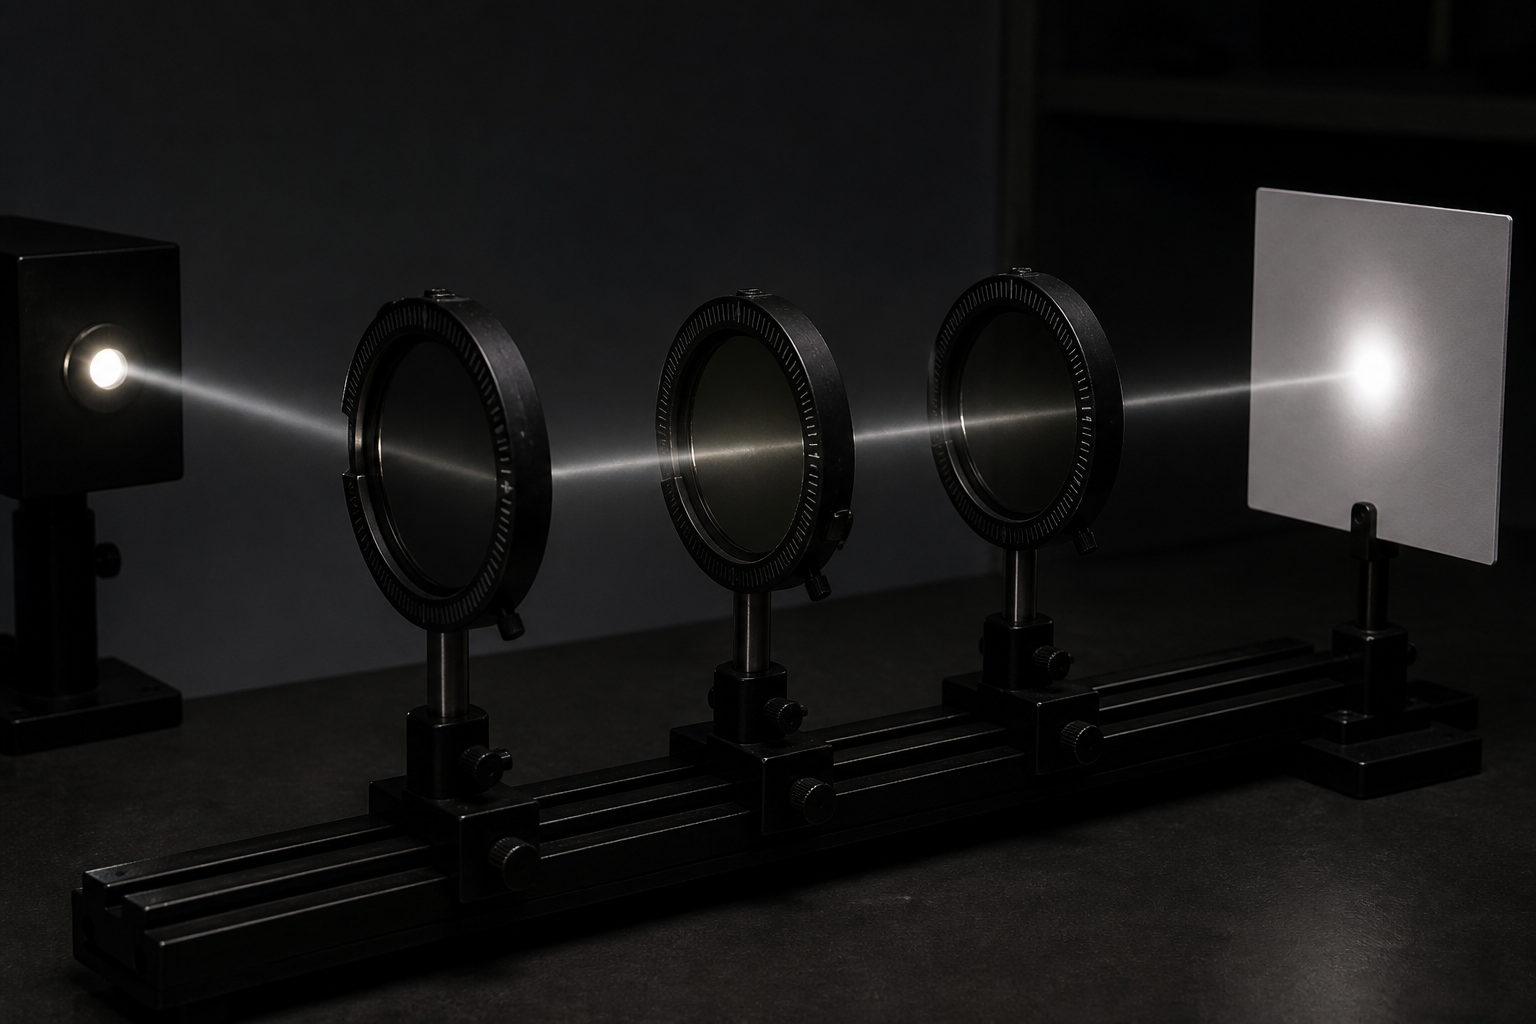
\includegraphics[width=0.58\linewidth]{images/book5/ai/b5-08-three-polarizers.png}

{\small ثلاثة مستقطِبات على منضدة: كل واحد منها قياس، يسقط حالة الضوء على محور. فقاطع بين اثنين لا يعبر شيء؛ ثم أدخل ثالثًا بينهما بزاوية يعود الضوء --- أي مسلَّمات هذا الفصل مؤدّاة على طاولة.}
\end{omfigure}

\section{تمارين}

\begin{exercise}[$\star$]\label{exo:b3:quantum-formalism:1}
في أساس متعامد نظامي $(\ket1, \ket2)$، لتكن $\ket\psi = (2\ket1 +
\iu\ket2)/\sqrt5$ و $\ket\varphi = (\ket1 - \ket2)/\sqrt2$. (أ)
تحقق من التنظيمين. (ب) احسب $\braket\varphi\psi$ و
$\braket\psi\varphi$. (ج) احسب احتمال إيجاد $\ket\psi$ في
الحالة $\ket\varphi$. (د) أنشئ الحالة المتعامدة مع
$\ket\psi$ (إلى طور).
\end{exercise}

\begin{exercise}[$\star$]\label{exo:b3:quantum-formalism:2}
أيّ هذه المصفوفات هرميتي، وما القيم الذاتية
والمتجهات الذاتية المنظَّمة لما هو كذلك؟
\[
\begin{pmatrix}0 & 1\\ 1 & 0\end{pmatrix} , \quad
\begin{pmatrix}0 & -\iu\\ \iu & 0\end{pmatrix} , \quad
\begin{pmatrix}1 & 1\\ -1 & 1\end{pmatrix} , \quad
\begin{pmatrix}2 & 1-\iu\\ 1+\iu & 3\end{pmatrix} .
\]
\end{exercise}

\begin{exercise}[$\star$]\label{exo:b3:quantum-formalism:3}
ضوء مستقطب بالزاوية $\alpha$ يلاقي محلّلًا بالزاوية
$\beta$. (أ) اكتب الحالتين في الأساس $(\ket H, \ket V)$ و
احسب احتمال النفوذ. (ب) استعد قانون مالوس. (ج)
من أجل سيل من $N$ فوتونًا، ما تباين العدد
النافذ؟ (د) ضوء دائري $(\ket H + \iu\ket V)/\sqrt2$ على محلّل
خطي بأيّ زاوية: ما النفوذ؟ فسّر استقلال الجواب
عن الزاوية.
\end{exercise}

\begin{exercise}[$\star$]\label{exo:b3:quantum-formalism:4}
(أ) برهن على أن $[\hat x, \hat p] = \iu\hbar$ بالتأثير في دالة اختبار.
(ب) احسب $[\hat x^2, \hat p]$ و $[\hat x, \hat p^2]$. (ج) بيّن أن
$[\hat A, \hat B\hat C] = [\hat A, \hat B]\hat C + \hat B[\hat A,
\hat C]$. (د) استنتج $[\hat x, \hat p^n] = \iu\hbar\,n\hat p^{n-1}$
وفسّر: أيّ عملية كلاسيكية يحاكيها $[\hat x, \cdot\,]$؟
\end{exercise}

\begin{exercise}[$\star\star$]\label{exo:b3:quantum-formalism:5}
قياسات متتالية. فوتون يبدأ في الحالة $\ket V$. (أ) يلاقي
مستقطِبين عند $45^\circ$ ثم $0^\circ$ (أفقي): احسب
احتمال نجاته من الاثنين، مع إظهار الانهيار الوسيط
صراحةً. (ب) استبدل بالمستقطِب الأوسط مستقطِبين عند $30^\circ$ و
$60^\circ$: ما النفوذ؟ (ج) ومع $N - 1$ مستقطِبًا وسيطًا
بخطوة $90^\circ/N$: بيّن أن احتمال النجاة هو
$\cos^{2N}(\pi/2N)$ وقدّره من أجل $N = 2, 5, 20$. (د) في النهاية
$N \to \infty$ يدور الاستقطاب من دون \emph{أيّ} خسارة:
علّق (وتُستعمل دورة ``زينون الكمومية'' هذه على كيوبتات حقيقية).
\end{exercise}

\begin{exercise}[$\star\star$]\label{exo:b3:quantum-formalism:6}
على فضاء المستويين، $\hat A = \begin{pmatrix}0&1\\1&0
\end{pmatrix}$ و $\hat B = \begin{pmatrix}1&0\\0&-1\end{pmatrix}$.
(أ) احسب $[\hat A, \hat B]$: أهما متوافقتان؟ (ب) الحالة هي
$\ket1$: أعطِ إحصاءات نتائج قياس $\hat B$، ثم
إحصاءات قياس $\hat A$ \emph{بعد} قياس $\hat B$ أعطى $+1$.
(ج) قِس $\hat A$ أولًا (والنتيجة $+1$)، ثم $\hat B$، ثم
$\hat A$ من جديد: بأيّ احتمال \emph{يناقض} قياس $\hat A$
الأخير الأولَ؟ (د) ماذا كانت \omterm{def:b3:quantum-formalism:commutator}{مبدّلة} معدومة ستقتضي في (ج)؟
\end{exercise}

\begin{exercise}[$\star\star$]\label{exo:b3:quantum-formalism:7}
(أ) من أجل الحالة الغاوسية في
\cref{exo:b3:schrodinger-three-dimensions:1} مقصورةً على بُعد
واحد، احسب $\Delta x$ و $\Delta p$ (باستعمال زوج فورييه أو
بالمكاملة) وتحقق من المساواة في علاقة هايزنبرغ. (ب) أيّ
الحالات تشبّع مبرهنة الارتياب العامة (اذكر الشرط
من حالة المساواة في كوشي--شوارتز)؟ (ج) إلكترون محصور في
$\Delta x = \qty{0.1}{nm}$: ما أدنى مقياس لطاقته الحركية؟ (د) والسؤال نفسه
من أجل كرية ($\qty{10}{g}$) موطَّنة إلى ميكرومتر: استنتج.
\end{exercise}

\begin{exercise}[$\star\star$]\label{exo:b3:quantum-formalism:8}
(أ) انطلاقًا من \cref{prop:b3:quantum-formalism:evolution}، استعد
زوج إهرنفست من أجل $\hat x$ و $\hat p$ مع $\hat H = \hat
p^2/2m + V$. (ب) بيّن أن الزوجية $\hat\Pi$ (حيث $\hat\Pi\psi(x) =
\psi(-x)$) هرميتية، ومربعها المطابقة، وقيمها
الذاتية $\pm1$. (ج) بيّن أن $[\hat H, \hat\Pi] = 0$ من أجل كمون
متناظر واستنتج أن للمستويات غير المنحلّة زوجية
محددة. (د) أيّ واقعة مشاهَدة عن مستويات بئر مزدوجة
متناظرة يفسّرها ذلك (تذكّر ثنائي النشادر في كتاب
السنة الثانية)؟
\end{exercise}

\begin{exercise}[$\star\star$]\label{exo:b3:quantum-formalism:9}
جملة تامة في العمل. في العلبة المربعة الثنائية البعد، يُولَّد المستوي $E
\propto 5$ بالحالتين $\ket{1,2}$ و $\ket{2,1}$. (أ) بيّن أن
الطاقة وحدها لا تسم الحالات. (ب) ليبدّل $\hat S$ المتغيرين $x
\leftrightarrow y$: بيّن أن $\hat S$ هرميتي ويتبادل مع $\hat
H$، وأوجد حالاته الذاتية داخل المستوي. (ج) تحقق من أن الزوج $(\hat H, \hat S)$ يسم
كل حالة من هذا المستوي وسمًا وحيدًا. (د) أعطِ العبرة العامة:
الانحلال يعني أن مجموعة الوسوم لم تكتمل بعد،
والتناظر يقدّم الوسم الناقص.
\end{exercise}

\begin{exercise}[$\star\star\star$]\label{exo:b3:quantum-formalism:10}
ارتياب الطاقة والزمن بأمانة. من أجل أيّ \omterm{def:b3:quantum-formalism:observable}{مرصودة} $\hat A$،
عرّف زمن التطور $\tau_A = \Delta A\,/\,|\dd\langle\hat
A\rangle/\dd t|$ --- وهو زمن انتقال المتوسط بانحراف معياري
واحد. (أ) انطلاقًا من \cref{thm:b3:quantum-formalism:uncertainty} و
\cref{prop:b3:quantum-formalism:evolution}، برهن على أن $\Delta
E\;\tau_A \ge \hbar/2$. (ب) لماذا \emph{ليس} هذا ارتيابًا
بين مرصودتين (فما الزمن، في الصياغة)؟ (ج) طبّقه
على حالة ذرية مثارة عمرها \qty{10}{ns}: احسب عرض الخط. (د)
طبّقه على ساعة معصمك: بأيّ حدّة يمكن أن تكون طاقة جملة إذا
تغيّر فيها شيء مرئي كل ثانية؟
\end{exercise}

\begin{exercise}[$\star\star\star$]\label{exo:b3:quantum-formalism:11}
برهان مبرهنة الارتياب. مع $\hat\alpha, \hat\beta$ كما في
النص: (أ) برّر $\Delta A^2 = \|\hat\alpha\ket\psi\|^2$ باستعمال
الهرميتية؛ (ب) طبّق كوشي--شوارتز واقسم
$\braket{\hat\alpha\psi}{\hat\beta\psi}$ إلى جزأين هرميتي و
مضاد هرميتي، وعيّنهما بمتوسطَي \omterm{def:b3:quantum-formalism:commutator}{المبدّلة} \omterm{def:b3:quantum-formalism:commutator}{والمبدّلة}
المضادّة؛ (ج) استنتج، واذكر متى تتحقق المساواة؛
(د) بيّن أنه من أجل $[\hat A, \hat B] = \iu\hbar$ لا يمكن لأيّ حالة أن تكون
متجهة ذاتية لأيّ من المرصودتين مع بقاء الانحرافين
منتهيين --- ووفّق ذلك مع الأمواج المستوية.
\end{exercise}

\begin{exercise}[$\star\star\star$]\label{exo:b3:quantum-formalism:12}
القِدر المراقَبة. جملة ذات مستويين تبدأ في $\ket1$ وتقود
هاميلتونيتها اهتزازًا شبيهًا باهتزاز رابي: فبعد الزمن $t$ تكون الحالة
$\cos(\omega t)\ket1 + \sin(\omega t)\ket2$ (خذ هذا معطى).
(أ) من دون أيّ قياس، متى يكتمل الانتقال إلى $\ket2$؟
(ب) قِس ``في أيّ حالة؟'' عند الأزمنة $T/N, 2T/N, \dots$ مع $T =
\pi/2\omega$: بيّن أن احتمال إيجاد الجملة
\emph{ما زالت} في $\ket1$ عند كل فحص هو $[\cos^2(\pi/2N)]^N$. (ج)
قدّره من أجل $N = 1, 4, 20, 100$ وبيّن أنه يؤول إلى $1$: فالمراقبة
المتواترة تجمّد التطور (وهو أثر زينون الكمومي،
المشاهَد بأيونات محصورة سنة 1990). (د) اشرح في جملة واحدة
أيّ مسلَّمة تقوم بالتجميد.
\end{exercise}

\begin{omfigure}
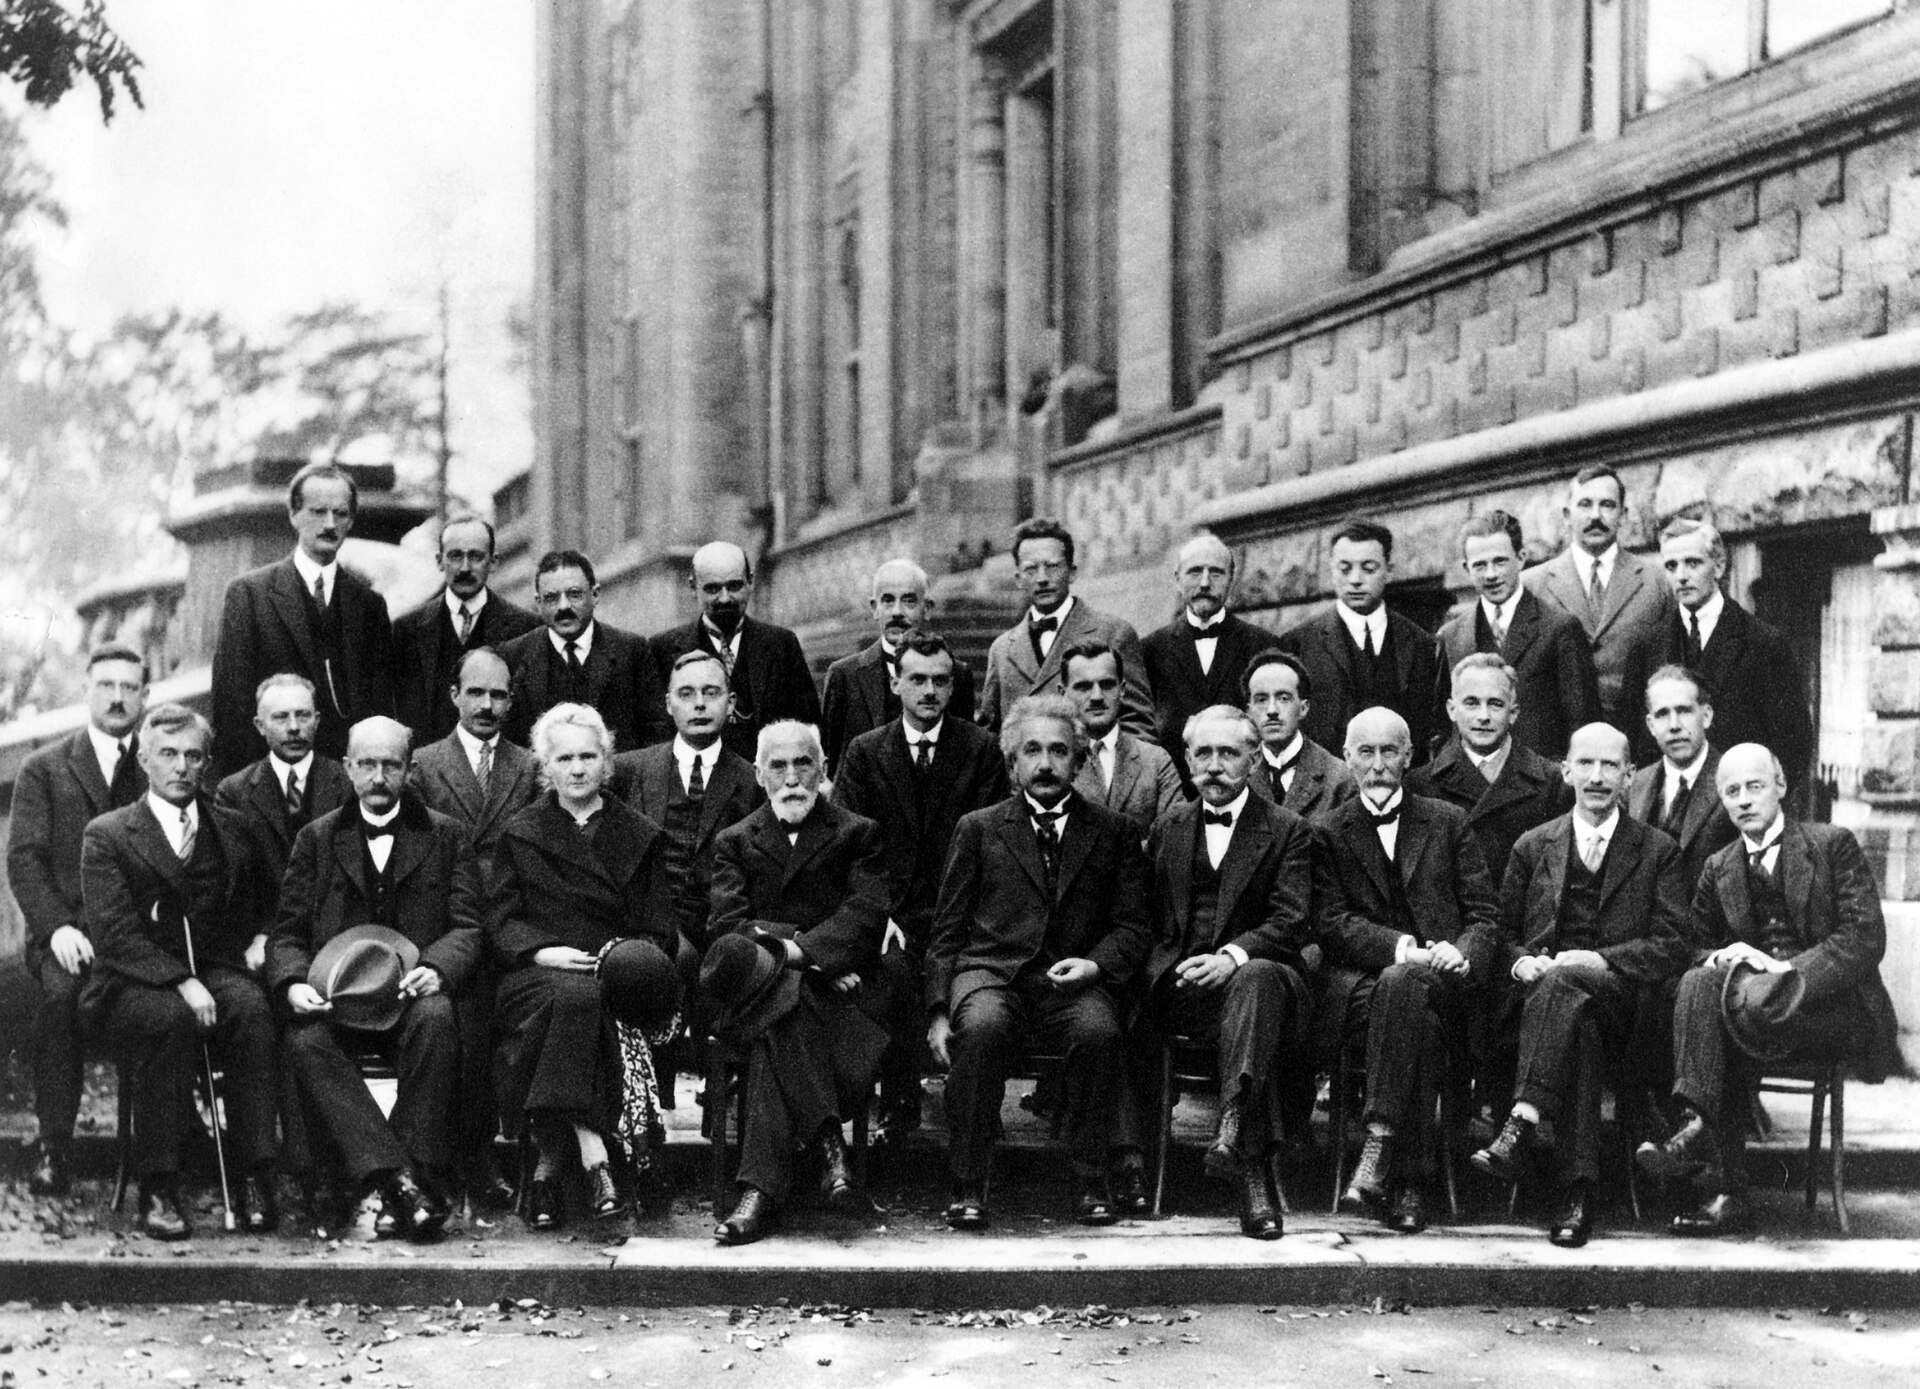
\includegraphics[width=0.62\linewidth]{images/book5/photo-solvay-1927.jpg}

{\small مؤتمر سولفاي سنة 1927 (صورة بعدسة بنجامان كوبري، ملك عام): من بنوا مسلَّمات هذا الفصل، في غرفة واحدة --- وهم لا يزالون يتجادلون، في ذلك الأسبوع نفسه، في معنى القياس.}
\end{omfigure}

\section{مسألة: النيوترينوات تبدّل ثيابها في الطيران}

\begin{problem}[{مسألة نهاية الأسبوع --- تذبذبات ذات مستويين عبر
الأرض}]\label{pb:b3:quantum-formalism:1}
تولد النيوترينوات في التفاعلات النووية حالاتِ \emph{نكهة} ---
نيوترينو إلكتروني $\ket{\nu_e}$ أو نيوترينو ميوني $\ket{\nu_\mu}$ ---
لكنها \emph{تنتشر} حالاتِ طاقة (أي كتلة) ذاتية $\ket{\nu_1},
\ket{\nu_2}$. والأساسان لا ينطبقان: بل بينهما دوران بزاوية
\emph{مزج} $\theta$،
\[
\ket{\nu_e} = \cos\theta\,\ket{\nu_1} + \sin\theta\,\ket{\nu_2} ,
\qquad
\ket{\nu_\mu} = -\sin\theta\,\ket{\nu_1} + \cos\theta\,\ket{\nu_2} .
\]
وقد نال اكتشافُ أن النيوترينوات \emph{تتذبذب} من ثمّ بين
النكهات --- ومن ثمّ أن لها كتلة --- جائزة نوبل لسنة 2015.
وتستنتج هذه المسألة الأثر بلا شيء وراء هذا
الفصل. فلنيوترينو فوق نسبي كمية حركته $p$ وكتلته
$m_i$ طاقة $E_i \approx pc + m_i^2c^4/2pc \approx E +
m_i^2c^4/2E$.

\medskip\noindent\textbf{الجزء الأول --- إعداد الصياغة.}
\begin{enumerate}
  \item تحقق من أن تعامد $(\ket{\nu_1}, \ket{\nu_2})$ ونظاميتهما يجعلان
        $(\ket{\nu_e}, \ket{\nu_\mu})$ متعامدين نظاميين أيضًا.
  \item لماذا يجب أن يكون أساس الانتشار هو الأساس الذاتي
        \emph{للطاقة}، مهما يكن الأساس الذي وُلد فيه النيوترينو؟ (فأيّ
        مسلَّمة تحكم الطيران الحر؟)
  \item يولد نيوترينو ميوني عند $t = 0$. اكتب $\ket{\psi(0)}$ في
        أساس الكتلة.
  \item اكتب $\ket{\psi(t)}$، وكل مركبة كتلية تحمل
        طورها $\eu^{-\iu E_it/\hbar}$.
  \item بيّن أن الطور \emph{الشامل} لا أثر له وأخرج
        $\eu^{-\iu E_1t/\hbar}$ عاملًا: فلا يقود الفيزياء إلا الطور \emph{النسبي}
        $\Delta\phi = (E_2 - E_1)t/\hbar$.
  \item عبّر عن $E_2 - E_1$ بدلالة $\Delta m^2 = m_2^2 - m_1^2$
        و $E$، من أجل نيوترينوات فوق نسبية.
\end{enumerate}

\medskip\noindent\textbf{الجزء الثاني --- صيغة التذبذب.}
\begin{enumerate}[resume]
  \item احسب السعة $\braket{\nu_e}{\psi(t)}$.
  \item بيّن أن احتمال الظهور هو
        \[
        \mathcal P_{\nu_\mu \to \nu_e}(t) =
        \sin^2(2\theta)\,\sin^2\Big(\frac{\Delta\phi}{2}\Big) .
        \]
        (استعمل $2\sin\theta\cos\theta = \sin2\theta$.)
  \item تحقق من الحالتين الحديتين: $\theta = 0$ و $m_1 = m_2$.
        فبم يبرهن إذًا أيّ تذبذب مشاهَد؟
  \item مع $t \approx L/c$، بيّن أن
        \[
        \mathcal P = \sin^2(2\theta)\,
        \sin^2\Big(\frac{\Delta m^2c^4}{4\hbar c}\,\frac{L}{E}\Big) ,
        \]
        وعرّف طول التذبذب $L_{\text{تذبذب}} =
        4\pi\hbar cE/\Delta m^2c^4$.
  \item بيّن أن احتمال النجاة $\mathcal P_{\nu_\mu \to
        \nu_\mu} = 1 - \mathcal P_{\nu_\mu\to\nu_e}$: فأين
        استُعملت الواحدية؟
  \item لماذا لا يقيس التذبذب إلا $\Delta m^2$، ولا يقيس
        الكتل نفسها أبدًا؟
\end{enumerate}

\medskip\noindent\textbf{الجزء الثالث --- قراءة التجارب.}
تمطر نيوترينوات ميونية جوّية ($E \approx \qty{1}{GeV}$) على
كاشف من الأعلى ($L \approx \qty{15}{km}$) ومن الأسفل،
عبر الأرض ($L \approx \qty{12800}{km}$). وقد وجدت تجربة سوبر-كاميوكاندي
(1998) التدفق الآتي من الأسفل منصَّفًا والآتي من الأعلى سليمًا.
\begin{enumerate}[resume]
  \item باستعمال $\hbar c = \qty{197}{MeV.fm}$، بيّن الصورة
        العملية $\dfrac{\Delta m^2c^4\,L}{4\hbar cE} = 1.27\,
        \dfrac{\Delta m^2c^4\,[\unit{eV^2}]\ L\,[\unit{km}]}
        {E\,[\unit{GeV}]}$.
  \item إذا كان التذبذب \emph{مكتمل النموّ} عند $L =
        \qty{12800}{km}$ و\emph{مهملًا} عند \qty{15}{km} من أجل
        $E = \qty{1}{GeV}$، فحاصر $\Delta m^2c^4$ تقريبًا.
  \item القيمة المقيسة $\Delta m^2c^4 \approx
        \qty{2.5e-3}{eV^2}$: احسب طول التذبذب عند
        \qty{1}{GeV} وتحقق منه أمام المسافتين.
  \item الكبت الآتي من الأسفل قريب من $1/2$، لا من $0$:
        بيّن أن \emph{توسيط} $\sin^2$ على أطوال تذبذب كثيرة
        (وعلى الطاقات) يعطي $\tfrac12\sin^22\theta$،
        واستنتج أن المزج الجوّي يكاد يكون
        \emph{أعظميًا} ($\theta \approx 45^\circ$).
  \item ماذا تعطي $\Delta m^2c^4 = \qty{2.5e-3}{eV^2}$ من أجل
        الكتلة الأثقل وحدها إذا كانت الأخفّ مهملة --- و
        قارن ذلك بكتلة الإلكترون: فما أغرب خفّة
        النيوترينوات!
  \item لمضادات النيوترينو المفاعلية $E \approx \qty{4}{MeV}$. وباستعمال
        صيغة $1.27$ نفسها، بيّن أن مسافة قاعدية من كيلومتر إلى
        كيلومترين موالَفة على الانفصام $\qty{2.5e-3}{eV^2}$
        (وهي تجربة دايا باي)، بينما $L \approx \qty{180}{km}$
        (تجربة كام-لاند) موالَفة على الانفصام ``الشمسي'' الأصغر
        $\qty{7.5e-5}{eV^2}$ --- تحقق من كليهما عدديًا.
\end{enumerate}

\medskip\noindent\textbf{الجزء الرابع --- ما معنى ذلك.}
\begin{enumerate}[resume]
  \item تصدر الشمس $\nu_e$؛ وطوال عقود لم تحصِ الكواشف إلا
        ثلث التنبؤ. اشرح ``مسألة النيوترينوات الشمسية''
        وحلّها، كلًّا في جملة واحدة.
  \item لماذا فرضت التذبذبات استنتاج أن للنيوترينوات
        \emph{كتلة}، خلافًا للحساب الأصلي في النموذج المعياري؟
  \item جملة كمومية تحفظ ترابط الطور على مدى
        $12800$ كيلومتر: فماذا يقول هذا عن مدى ضعف تفاعل
        النيوترينوات، ولماذا يجب أن يكون الكاشف هائلًا؟
  \item النكهة \omterm{def:b3:quantum-formalism:observable}{مرصودة}: فلماذا لا يتبادل مؤثرها مع
        \omterm{def:b3:hamiltonian-mechanics:hamiltonian}{الهاميلتونية} الحرة، وأيّ قانون انحفاظ \emph{لا}
        يتوفر إذًا للنكهة (بينما تبقى الطاقة وكمية الحركة
        محفوظتين)؟
  \item للطبيعة ثلاث نكهات وثلاث كتل: فلماذا تصف مع ذلك
        المعالجة ذات المستويين كل تجربة وصفًا
        جيدًا؟ (انظر في تراتب المقدارين $\Delta m^2$
        وأيّهما تفصله كل مسافة قاعدية.)
  \item في صياغة هذا الفصل، سمِّ بالضبط أيّ المكوّنات
        أنتجت التذبذب: أيّ عدم تطابق بين أساسين،
        وأيّ مسلَّمة، وأيّ طور.
  \item لخّص النتيجة الموسومة: زاوية دوران قرب
        $45^\circ$ وانفصام $\Delta m^2c^4 =
        \qty{2.5e-3}{eV^2}$ يجعلان نيوترينو ميونيًا بالجيغا إلكترون-فولط يختفي بطول
        تذبذب $\sim\qty{1000}{km}$ --- أي جبر خطي ذي مستويين،
        مؤكَّدًا عبر جسم الأرض.
\end{enumerate}
\end{problem}
